%%%%%%%%%%%%%%%%%%%%%%%%%%%%%%%%%%%%%%%%%
%%%%%%%%%%%%%%%%%%%%%%%%%%%%%%%%%%%%%%%%%
% Thin Sectioned Essay
% LaTeX Template
% Version 1.0 (3/8/13)
%
% This template has been downloaded from:
% http://www.LaTeXTemplates.com
%
% Original Author:
% Nicolas Diaz (nsdiaz@uc.cl) with extensive modifications by:
% Vel (vel@latextemplates.com)
%
% License:
% CC BY-NC-SA 3.0 (http://creativecommons.org/licenses/by-nc-sa/3.0/)
%
%%%%%%%%%%%%%%%%%%%%%%%%%%%%%%%%%%%%%%%%%

%----------------------------------------------------------------------------------------
% PACKAGES AND OTHER DOCUMENT CONFIGURATIONS
%----------------------------------------------------------------------------------------

\documentclass[a4paper, 11pt]{article} % Font size (can be 10pt, 11pt or 12pt) and paper size (remove a4paper for US letter paper)

\usepackage[protrusion=true,expansion=true]{microtype} % Better typography
\usepackage[utf8]{inputenc}  
\usepackage{graphicx} % Required for including pictures
\usepackage{wrapfig} % Allows in-line images
\usepackage[a4paper, margin={3cm, 3cm}]{geometry}

\usepackage{mathenv}
\usepackage{amsmath,amsfonts,amssymb}
\usepackage{setspace}
\usepackage{bbm}
\usepackage{bm}
\usepackage{layout}
\usepackage[]{algorithm2e}

\usepackage{mathpazo} % Use the Palatino font
\usepackage[T1]{fontenc} % Required for accented characters
\linespread{1.05} % Change line spacing here, Palatino benefits from a slight increase by default

\usepackage{listings} % Pour ajouter du code
\usepackage{xcolor}
\lstset { %
    language=C++,
    backgroundcolor=\color{black!5}, % set backgroundcolor
    basicstyle=\footnotesize,% basic font setting
}

\makeatletter
\renewcommand\@biblabel[1]{\textbf{#1.}} % Change the square brackets for each bibliography item from '[1]' to '1.'
\renewcommand{\@listI}{\itemsep=0pt} % Reduce the space between items in the itemize and enumerate environments and the bibliography

\renewcommand{\maketitle}{ % Customize the title - do not edit title and author name here, see the TITLE block below
\begin{flushright} % Right align
{\LARGE\@title} % Increase the font size of the title

\vspace{30pt} % Some vertical space between the title and author name

{\large\@author} % Author name
\\\@date % Date

\vspace{20pt} % Some vertical space between the author block and abstract
\end{flushright}
}

%----------------------------------------------------------------------------------------
% TITLE
%----------------------------------------------------------------------------------------

\title{\textbf{Projet Velib : Equilibrage nocturne d'un parc de vélos}\\ % Title
C9-4} % Subtitle

\author{\textsc{ARFAOUI Armani, Jay Emmanuel, Dufour Maxime} % Author
\\{\textit{ENSTA ParisTech}}} % Institution

\date{\today} % Date

%----------------------------------------------------------------------------------------

\begin{document}

\vspace{200pt}

\maketitle % Print the title section

\section{Réalisation de la brique d'équilibrage}

\paragraph*{}
Cette première étape consiste à implémenter une brique d'équilibrage performante pour un circuit donné. C'est-à-dire calculer la charge initiale à déposer dans la remorque utilisée pour ce circuit puis les dépôts/charges effectués en chaque station du circuit.

\subsection{Fonctionnement de la brique d'équilibrage}

\paragraph*{}
On peut d'hors et déjà remarquer que la pénalisation du déséquilibre en une station est indépendante de la station étudiée. Le déséquilibre dans deux stations différentes est évalué de la même manière du point de vue de la qualité de la solution trouvée. Pour un circuit donné, il est alors équivalent de traiter le déséquilibre des premières stations du circuit en priorité ou bien de traiter celui des dernières stations du circuit. Traiter en priorité les premières stations du circuit semblant plus simple, la démarche gloutonne consistant pour la remorque à ré-équilibrer au mieux les stations au fur et à mesure de leur visite semble tout indiquée. Nous avons construit une fonction équilibrate qui se déroule en deux temps. D'abord, elle calcule la charge initiale optimale puis elle assigne à chaque station le meilleur depôt (positif ou non) possible. 

\paragraph*{}
Calcul de la charge intiale: Inititalement, on autorise la charge initiale à prendre ses valeurs entre 0 (borne minimale) et la capacité maximale (borne maximale) de la remorque puis au fur et à mesure du parcours des stations, on restreint de plus en plus ses bornes jusqu'à ce qu'elle ne puisse plus tenir. A chaque fois que l'on quitte une station, on calcule la charge courante de la remorque comme somme des charges (un dépôt étant compté négativement) effectuées jusqu'à quitter cette station. Si la charge courante est supérieure à la borne minimale c'est qu'il faut mettre la borne minimale à jour pour pouvoir satisfaire le déséquilibre des stations parcourues et la fixer égale à la valeur courante. La mise à jour de la borne supérieure est un peu plus complexe, il s'agit ici de détecter si l'on a emporté trop de vélos inititalement. On compare donc la charge courante à la différence entre la borne maximale et la capacité de la remorque. Si la charge courante est inférieure à cette valeur (i.e. charge courante < charge maximale - remorque->capa, ce qui implique qu'elle soit négative pour modifier la borne maximale) alors on met à jour la borne maximale (charge maximale = charge courante + remorque->capa, qui est bien inférieure a remorque->capa puisque la charge courante est négative lorsque l'on met à jour la borne). On procède ainsi jusqu'à ce que la borne minimale soit supérieure ou égale à la borne maximale, dans ce cas on ne peut plus modifier la charge intiale de manière à mieux satisfaire le déséquilibre des stations parcourues. On fixe donc la valeur de la charge intiale à la valeur de la borne qui n'a pas été modifiée à la dernière itération (i.e. la dernière station atteinte) et on a la charge initiale optimale permettant de satisfaire au mieux les stations atteintes avant le croisement des bornes minimales et maximales (ce qui est l'optimum sur le circuit dans sa gloabalité puisque nous avons montré dans le paragraphe précédent qu'il était équivalent de traiter les déséquilibres au fur et à mesure du parcours des stations).

\paragraph*{}
Calcul du dépôt en chaque station: On a déjà calculé la charge initiale optimale dans la première partie de la brique équilibrate. On parcourt de nouveau les station du circuit. Tant que la charge le permet, on compense parfaitement le déséquilibre. Dès que l'on doit déposer plus de vélos que l'on en a dans la remorque, on dépose tout ce qu'on peut (le déséquilibre global du circuit est incrémenté) et on obtient une remorque vide qui continue son trajet (peut-être qu'ultérieurement elle récupérera des vélos qu'elle pourra redéposer). Si l'on doit récupérer plus de vélos plus que l'on a de places libres dans la remorque, on recupère tout ce que l'on peut (le déséquilibre global du circuit est incrémenté) et l'on obtient une remorque pleine qui continue également son trajet (de la même manière elle rencontrera peut-être une station nécessitant un dépôt ultérieurement dans son circuit). De cette manière, on a un dépôt optimal en chaque station pour le circuit considéré.



\subsection{Questions subsidiaires}

\paragraph*{}
Si le coût de pénalité était linéaire et différent selon les stations, il faudrait équilibrer en priorité les stations de coût maximal. Ce n'est pas évident à réaliser si elles ne sont pas situées au début du circuit avec la méthode gloutonne que nous avons décrit précédemment. Dans ce cas, une première approche serait simplement de trier les stations du circuit par coût de pénalisation pour commencer par équilibrer en priorité celles dont le coût est le plus élevé. Avec cette approche, on ne tient pas vraiment compte de l'ordre de parcours des stations mais comme la distance parcourue est bien moins pénalisée que le déséquilibre, il est réellement intéressant de prioriser celui-ci lors du calcul d'une solution. On ordonne donc les stations en  fonction de leur coût dans la fonction objectif et on chercher à équilibrer en priorité les stations avec les coûts les plus élevés.

\paragraph*{}
Si la pénalisation est non linéaire, la méthode employée dépendra grandement de la fonction coût utilisée. Par exemple, si l'on sélectionne une pénalisation quadratique. L'équilibrage devra être le plus diffus possible pour éviter des cas où une station serait très déséquilibrée (grosse pénalisation) alors que toutes les autres stations sont équilibrées. Il faudrait mieux créer des solutions dans lesquelles toutes les stations ont un léger déséquilibrage pour minimiser la fonction objectif. Pour cela on pourrait calculer un indicateur donnant le déséquilibre initiale du circuit et ainsi obtenir un déséquilibre moyen que l'on doit obtenir pour les stations du circuit.

\section{Glouton intelligent}

\paragraph*{}
Dans cette étape, nous allons réaliser un glouton intelligent utilisant les deux briques de base (équilibrage et insertion). Pour cela nous avons comparé différentes méthodes plus ou moins intelligentes pour mieux comprendre l'impact d'appels trop fréquents à ces briques de base. Chacune de ces méthodes repose sur un tri préalable des stations en fonction de leur déficit. L'idée de notre algorithme glouton est de sélectionner successivement le premier et le dernier élément de la liste pour que les déséquilibres se compensent au mieux (cela ne permettra pas forcément d'obtenir un déséquilibre nul si les deux extrêmes ont des valeurs absolues trop différentes). L'objectif principal à ce stade est de minimiser le déséquilibre sans prendre en compte la pénalité liée au trajet puisque le déséquilibre est nettement plus pénalisée. Pour le moment, on se contente d'assigner la quasi-totalité des stations à la remorque de plus grande capacité (en s'assurant d'assigner au moins une station à chaque remorque à la fin lorsque les déséquilibres sont les plus faibles pour s'assurer du respect des capacités des remorques). Les options ont été mises à jour pour pouvoir jongler au mieux entre les différentes techniques présentées ci-dessous.

\subsection{Utilisation exclusive du pushback}

\paragraph*{}
Cette première approche gloutonne pour exploiter la liste des stations triées par deficit sélectionne successivement le premier et le dernier élément de la liste triée et le place en bout de circuit. Cela ne nécessite quasiment aucun calculs pour placer une station et permet d'obtenir des solutions nettement meilleurs que le glouton stupide pour un temps de calcul instantané sur toutes les instances.

\paragraph*{}
L'intérêt de cette méthode est sa rapidité d'exécution pour trouver une solution améliorant nettement celle du glonton stupide. La piste d'amélioration porte sur l'insertion d'une station qui pour le moment est simpliste.

\subsection{Insertion exclusive avec insertbest}

\paragraph*{}
On continue d'exploiter la liste triée des stations en sélectionnant successivement le premier et le dernier élément de la liste. La différence principale est que l'insertion de la station sélectionnée se fait au moyen d'insertbest. On place optimalement la station dans le circuit existant ce qui peut permettre de comprenser des écarts trop grands entre deux bornes successives.

\paragraph*{}
Cette méthode est nettement plus longue (prend jusqu'à 3 minutes sur v9, la précédente méthode étant instantanée) mais permet de réduire le déséquilibre de manière notable.

\subsection{Insertion intelligente avec minimisation de l'appel à insertbest}

\paragraph*{}
Pour ne pas trop perdre en temps de calcul lors de l'insertion des stations, celle-ci va être réalisée en plusieurs étapes. Tout d'abord, on sélectionne une station (toujours une extrémité de la liste triée par déficit) puis on la place en bout de circuit. Si le déséquilibre du circuit correpondant est nul, on passe à la station suivante. Sinon, on retire la station du bout du circuit et on essaye de l'insérer au moyen d'insertbest. De la même manière si le déséquilibre du circuit est nul, on passe à la station suivante, sinon on place la station dans la deuxième remorque de plus grande capacité. On réitère ce procédé pour toutes les stations en s'assurant que toutes les remorques aient au minimum une station à visiter.

\paragraph*{}
Cette méthode permet d'obtenir des résultats très intéressant du point de vue de la minimisation du déséquilibre. Par ailleurs, le temps de calcul n'est pas trop long puisqu'on limite énormément l'appel à la fonction insertbest.

\paragraph*{}
Voici un récapitulatif des résultats comparant les trois différentes méthodes utilisées:
\begin{center}
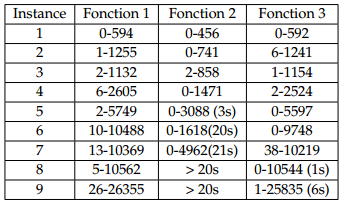
\includegraphics{glouton.png}
\end{center}




\section{Recuit simulé}

\paragraph*{}
Dans cette étape, on implémente un recuit simulé de la forme suivante :

\begin{center}
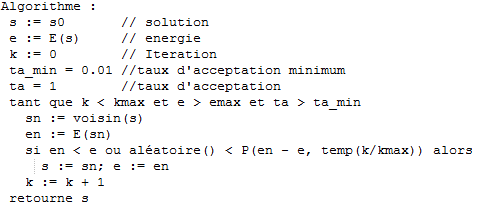
\includegraphics{recuit.png}
\end{center}

 %* Algorithme :
 %*  s := s0       // solution
 %*  e := E(s)     // energie
 %*  k := 0        // Iteration
 %*  ta_min = 0.01 //taux d'acceptation minimum
 %*  ta = 1        //taux d'acceptation
 %*  tant que k < kmax et e > emax et ta > ta_min
 %*    sn := voisin(s)
 %*    en := E(sn)
 %*    si en < e ou aléatoire() < P(en - e, temp(k/kmax)) alors
 %*      s := sn; e := en
 %*    k := k + 1
 %*  retourne s

\paragraph*{}
Dans un premier temps il convient de discuter de la méthode de voisinage utilisée pour parcourir l'ensemble des solutions. Notre première idée a été de sélectionner aléatoirement une station dans l'une des remorques. On la place ensuite au mieux avec insertbest dans une remorque choisie aléatoirement (pas nécessairement différente puisque la station n'était pas forcément au meilleur endroit dans la remorque). Le problème de cette méthode est tout d'abord son coût en terme de temps de calcul (insertbest est relativement lourd lors de multiples appels) et également le fait que peu de liberté est laissée au solveur pour parcours l'espace des solutions. C'est pourquoi nous avons construis un deuxième voisinage plus large, on sélectionne aléatoirement une station que l'on repositionne aléatoirement dans un des circuits. Cette méthode est rapide et permet un parcours facile de l'espace des solutions. Les options permettent de choisir l'un ou l'autre des voisinages, le guide des options ayant été mis à jour.

\paragraph*{}
La construction de la solution initiale se fait au moyen du glouton stupide qui permet l'obtention d'une solution rapide. Il faut évidemment faire attention au fait de ne pas sélectionner une station si c'est la seule de la remorque pour garder une solution admissible en partant de la solution admissible du glouton stupide (et ce pour les deux voisinages). Partir d'une solution a priori mauvaise n'est pas un problème, il suffit de paramétrer proprement le recuit simulé pour parcourir l'ensemble des solutions de manière satisfaisante avant de chercher à plonger dans un minimum.

\paragraph*{}
Nous avons donc définit notre solution initiale ainsi que notre voisinage. On utilise un pas géométrique dans un premier temps pour mettre à jour la température. Il faut maintenant déterminer les différents paramètres. Voilà un premier jeu de paramètre que nous avons mis en place:
\begin{itemize}
\item Taux d'acceptation minimal: 0.01
\item Nombre d'itérations: 100000 (obtention d'une solution avec 0 de déséquilibre plus rapide mais ce nombre d'itération permet de nettement améliorer le coût lié à la distance)
\item Température initiale : 100 000 000 (parcours immense des solutions au départ)
\item Coefficient de mise à jour de la température : 0.99 
\item Taille d'un palier de température : 15 (permet de diminuer rapidement la température pour éviter de continuer à parcours un espace des solutions trop grand)
\end{itemize}

\paragraph*{}
Le choix d'une grande température initiale permet un large parcours de l'espace des solutions pour commencer puis la mise à jour de la température sur de petits paliers permet de cibler rapidement de meilleurs solutions.

\paragraph*{}
Voici les premiers résultats que nous avons obtenus. On fixe le nombre d'itérations à 100000 donc le temps de calcul est délibéremment grand (le temps de calcul ne dépassant pas les 7 minutes pour v9). On s'attaque ici à un optimum global, sachant qu'un déséquilibre nul est trouvé bien avant le nombre d'itération maximal, on travaille énormément sur le coût des trajets en terme de distance.

\begin{center}
\begin{tabular}{|c|c|}
 \hline 
 Instance & Fonction objectif \\ \hline
 v0 &  0-355\\ \hline
 v1 &  0-335\\ \hline
 v2 &  0-537\\ \hline
 v3 &  0-598 \\ \hline
 v4 &  0-1456 \\ \hline
 v5 &  0-2743 \\ \hline
 v6 &  0-1951 \\ \hline
 v7 &  0-5507\\ \hline
 v8 &  0-10554\\ \hline
 v9 &  1-16375\\ \hline

\end{tabular}
\end{center}

On a le tracé de l'énergie en fonction de l'itération pour v9 avec deux paliers de température différents:
\begin{center}

\begin{figure}
\caption{température de v9 avec un palier de 10}
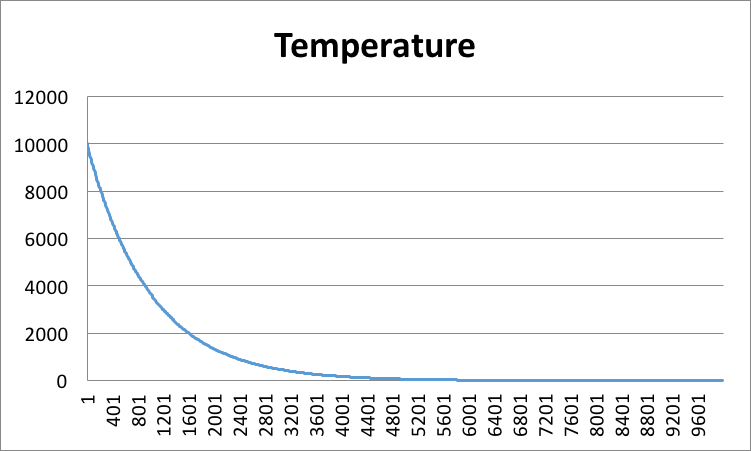
\includegraphics{v9-p10-it10000-temp.png}
\end{figure}

\begin{figure}
\caption{energie v9 avec un palier de 10}
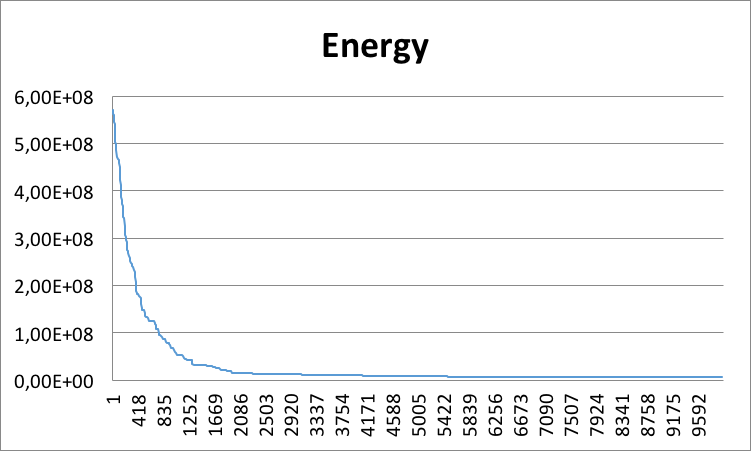
\includegraphics{v9-p10-it10000-energy.png}
\end{figure}

\end{center}

De plus amples résultats seront présentés pour vendredi.
\end{document}

